\chapter{Appendix}
\section{Feature map normalization}\label{appendix:new_feature}

\begin{lemma}
    Associated to any RKHS $\mathcal{H}$, there exists a feature vector $\phi(x)$ such that $\|\phi(x)\|_{\mathcal{H}}=R \quad \forall x \in \mathcal{X}$.
    That is the Hilbert space norm of the feature vector is equal to a constant R for all states in the set $\mathcal{X}$.
\end{lemma}
\begin{proof}
    Taking the new feature vector as $\phi^{new} (x):=\frac{\phi(x)}{\|\phi(x)\|_{\mathcal{H}}}$ we have
\begin{align*}
    \|
    \phi^{new}(x)\|_{\mathcal{H}}^{2} &= \left\|\frac{\phi(x)}{\|\phi(x)\|_{\mathcal{H}}}
    \right\|_{\mathcal{H}}^{2}
    \\
    &=
    \left\|
    \frac{\phi(x)}
    {\sqrt{k(x,x)}}
    \right\|_{\mathcal{H}}^{2}
    \\
    &=
    \left\langle
    \frac{\phi(x)}
    {\sqrt{k(x,x)}}
    ,
    \frac{\phi(x)}
    {\sqrt{k(x,x)}}
    \right\rangle_{\mathcal{H}}
    \\
    &=
    \frac{1}{\sqrt{k(x,x)^{2}}}
    \langle
    \phi(x)
    ,
    \phi(x)
    \rangle_{\mathcal{H}}
    \\
    &=1
\end{align*}
\end{proof}



\section{Quantile regressor extensive comparison}\label{appendix:quantile_regressor_extensive_comparison}
This section contains extensive comparison between our kernel quantile regression and other state of the art quantile regressors. We benchmark it on popular machine learning datasets.
\subsection{Boston housing dataset}
The Boston housing dataset \href{https://www.kaggle.com/datasets/altavish/boston-housing-dataset}{https://www.kaggle.com/datasets/altavish/boston-housing-dataset} contains information about various attributes for suburbs in Boston.
There are 13 indipendent variables:
\begin{itemize}
\item CRIM per capita crime rate by town
\item ZN proportion of residential land zoned for lots over 25,000 sq.ft.\
\item INDUS proportion of non-retail business acres per town
\item CHAS Charles River dummy variable (1 if tract bounds river; 0 otherwise)
\item NOX nitric oxides concentration (parts per 10 million)
\item RM average number of rooms per dwelling
\item AGE proportion of owner-occupied units built prior to 1940
\item DIS weighted distances to five Boston employment centres
\item RAD index of accessibility to radial highways
\item TAX full-value property-tax rate per 10,000
\item PTRATIO pupil-teacher ratio by town
\item B $1000(Bk - 0.63)^2$ where Bk is the proportion of afroamericans by town
\item LSTAT lower status of the population
\end{itemize}
The dependent variable is MEDV, that is the median value of owner occupied homes in \$1000's

\begin{table}
\caption{Pinball loss for Boston housing data}
\begin{tabular}{lllll}
\toprule
    & Linear qr & Gbm qr & Quantile forest & KQR \\
\midrule
CRPS & 1.3785678 & 1.1418540 & 1.0587686 & \textbf{1.0297572} \\
\bottomrule
\end{tabular}
\end{table}

\begin{table}
    \caption{Pinball loss quantile-wise for Boston data}
\begin{tabular}{lllll}
\toprule
    & Linear qr & Gbm qr & Quantile forest & KQR \\
\midrule
0.1 & 0.729749 & 0.771714 & 0.588441 & \textbf{0.578898} \\
0.2 & 1.122582 & 1.033442 & 0.932824 & \textbf{0.869145} \\
0.3 & 1.479486 & 1.170642 & 1.153765 & \textbf{1.142783} \\
0.4 & 1.712577 & 1.436263 & 1.352667 & \textbf{1.331955} \\
0.5 & 1.911385 & \textbf{1.344361} & 1.408333 & 1.396300 \\
0.6 & 1.989514 & 1.448885 & 1.464902 & \textbf{1.431705} \\
0.7 & 1.938362 & 1.508741 & 1.427912 & \textbf{1.382772} \\
0.8 & 1.658058 & 1.497901 & 1.275059 & \textbf{1.245288} \\
0.9 & 1.243965 & 1.206591 & 0.983784 & \textbf{0.918725} \\
\bottomrule
\end{tabular}
\end{table}
        
\begin{table}
\caption{Mean absolute error for Boston data}    
\begin{tabular}{lllll}
\toprule
    & Linear qr & Gbm qr & Quantile forest & Kernel qr \\
\midrule
 & 3.826326 & 2.845989 & 2.965490 & \textbf{2.810494} \\
\bottomrule
\end{tabular}

\end{table}

\subsection{Abalone dataset}
The abalone data \href{https://archive.ics.uci.edu/dataset/1/abalone}{https://archive.ics.uci.edu/dataset/1/abalone} consist of measurements of abalone molluscs, the goal is predicting their age by building a model for estimating its number of rings; age is the number of rings plus 1.5
The data has 8 attributes:
\begin{itemize}
    \item Sex Categorical variable either male, female or infant
    \item Length
    \item Diameter
    \item Height
    \item Whole height
    \item Shucked height
    \item Viscera weight
    \item Shell weight
\end{itemize}

\begin{table}
    \caption{Pinball loss for Abalone data}
\begin{tabular}{lllll}
    \toprule
     & Linear qr & Gbm qr & Quantile forest & KQR \\
    \midrule
    CRPS & 0.5613975 & 0.5531938 & \textbf{0.5212990} & 0.5252491 \\
    \bottomrule
    \end{tabular}
\end{table}
    
\begin{table}
    \caption{Pinball loss quantile-wise for Abalone data}
    \begin{tabular}{lllll}
    \toprule
     & Linear qr & Gbm qr & Quantile forest & KQR \\
    \midrule
    0.1 & 0.277903 & 0.290531 & 0.274079 & \textbf{0.269287} \\
    0.2 & 0.469361 & 0.488079 & \textbf{0.453110} & 0.457286 \\
    0.3 & 0.621961 & 0.625633 & \textbf{0.580766} & 0.596791 \\
    0.4 & 0.729757 & 0.715875 & \textbf{0.689904} & 0.691310 \\
    0.5 & 0.794695 & 0.766185 & \textbf{0.735945} & 0.740834 \\
    0.6 & 0.810691 & 0.785769 & \textbf{0.744928} & 0.746636 \\
    0.7 & 0.769587 & 0.730318 & \textbf{0.700287} & 0.710392 \\
    0.8 & 0.667776 & 0.656913 & 0.609378 & \textbf{0.608334} \\
    0.9 & 0.472244 & 0.472635 & \textbf{0.424593} & 0.431621 \\
    \bottomrule
    \end{tabular}
\end{table}
    
\begin{table}
    \caption{Mean absolute error for Abalone data}
    \begin{tabular}{lllll}
    \toprule
     & Linear qr & Gbm qr & Quantile forest & KQR \\
    \midrule
     & 1.627627 & 1.574179 & 1.499522 & \textbf{1.498583} \\
    \bottomrule
    \end{tabular}
\end{table} 

\subsection{Vehicle dataset}
This data contains info about used cars \href{https://www.kaggle.com/datasets/nehalbirla/vehicle-dataset-from-cardekho}{https://www.kaggle.com/datasets/ne-halbirla/vehicle-dataset-from-cardekho}, the predictors are:
\begin{itemize}
    \item Year
    \item Present\_price ex showroom price
    \item Kms Driven
    \item Fuel type
    \item Seller type
    \item Transmission
    \item Owner number of previous owners
\end{itemize}
The dependent variable is the selling price.

\begin{table}
\caption{Pinball loss for Vehicle data}
\begin{tabular}{lllll}
    \toprule
     & Linear qr & Gbm qr & Quantile forest & KQR \\
    \midrule
    CRPS & 0.4054449 & 0.2289554 & 0.2844410 & \textbf{0.2204343} \\
    \bottomrule
    \end{tabular}
\end{table}

\begin{table}
    \caption{Pinball loss quantile-wise for Vehicle data}
    \begin{tabular}{lllll}
    \toprule
     & Linear qr & Gbm qr & Quantile forest & KQR \\
    \midrule
    0.1 & 0.254649 & \textbf{0.139849} & 0.170489 & 0.182490 \\
    0.2 & 0.403772 & 0.236339 & 0.285875 & \textbf{0.223165} \\
    0.3 & 0.548820 & 0.244086 & 0.357375 & \textbf{0.242963} \\
    0.4 & 0.576918 & 0.263169 & 0.389305 & \textbf{0.262835} \\
    0.5 & 0.554367 & 0.306123 & 0.410738 & \textbf{0.295878} \\
    0.6 & 0.563046 & 0.335363 & 0.398125 & \textbf{0.306062} \\
    0.7 & 0.516019 & 0.287490 & 0.326572 & \textbf{0.283716} \\
    0.8 & 0.407742 & 0.261882 & 0.313698 & \textbf{0.235793} \\
    0.9 & 0.229115 & 0.215253 & 0.192233 & \textbf{0.171440} \\
    \bottomrule
    \end{tabular}
\end{table}

\begin{table}
    \caption{Mean absolute error for Vehicle data}
    \begin{tabular}{lllll}
    \toprule
     & Linear qr & Gbm qr & Quantile forest & KQR \\
    \midrule
     & 1.117714 & 0.606971 & 0.752197 & \textbf{0.594292} \\
    \bottomrule
    \end{tabular}
\end{table}
What can be concluded from these numerical examples is that, on average kernel quantile regression yields better results than quantile forest \cite{meinshausen2006quantile} and gradient boosting machine quantile regression \cite {friedman2001greedy} in terms of the pinball loss as well as in terms of the mean absolute error.



\section{Cross validation}\label{appendix:cross_validation}
Cross validation directly estimates the expected test error
\begin{equation}
    Err=\mathbb{E}\left[L\left(Y,\hat{f}(X)\right)\right]=\mathbb{E}\left[Err_{\Tau}\right]
\end{equation}
$Err_{\Tau}$ is the prediction error over an independent test sample
\begin{equation}
    \mathbb{E}_{\Tau}=\mathbb{E}\left[L\left(Y,\hat{f}(X)\right)| \Tau \right]
\end{equation}
that is, $Err$ is the average over everything that is random: X,Y and the training set $\Tau$ used to learn $\hat{f}$. Hence, our interest lies in estimating the $Err$ quantity in order to guide model selection.
\subsection{K-fold cross validation}
K-fold cross validation splits the data into $K$ roughly equally sized parts, then $K$ models are trained. For $k$ from 1 to $K$ we train the kth model on the whole dataset except the kth partition. Next,  the prediction error of the kth fitted model is computed. Finally averaging all the $k$ prediction erros we obtain an estimate for the expected test error. We select the model which performs best in terms of expected prediction error.
\\
Usually, $K$ is set equal to 5 or 10. Leave-one-out cross validation is the case when $K$ is set equal to the size of the data.
% REMEMBER: Parameters allow the model to learn the rules from the data while hyperparameters control how the model is training. Parameters learn their own values from data. In contrast, hyperparameters do not learn their values from data. We need to manually specify them before training the model
\subsection{Gridsearch}
Model performance depends higly on the choice of hyperparameters. Notice, there is no way to get to know them in advance, therefore, all we can do is trying a lot of combinations until we fit a good enough set of hyperparameters. Essentially, gridsearch carries out hyperparameter tuning by performing a search over a predefined hyperparemeters grid. During its search, it tries all possible combinations and evaluates the different models %(different hyperparameters define different models)
using cross validation. For example, suppose that the grid contains 100 possible candidates and that we are doing 5-fold cross-validation, then the gridsearch algorithm will carry out 500 iterations.
Therefore, we get an estimate of prediction error for each considered model and this guides us in the hyperparameters selection.

\subsection{Randomized search}
Randomized search controls the number of steps by choosing smartly the hyperparameters to try in each iterations.
Let us say, there are 100 candidates and we set the number of iterations to 20 then the search will stop after the 20th iteration and return the best set among the hyperparameters observed.
The advantage is that it is much more quicker than gridsearch, but on the other hand its performance is worse than gridsearch.

\subsection{Halving gridsearch}
Gridsearch has been the to go choice for hyperparameters tuning for the past years. However, such method is brute forcing all possible combinations, hence it is highly computationally intensive, especially when it comes to large datasets.
\\
The scikit-learn team addressed this disadvantage of gridsearch by introducing the halving gridsearch method \citeW{scikithalvinggridsearch} (2020). Such technique has proved itself to greatly speed up hyperparameter tuning.
The ground concept underlying this method is successive halving. During the first iteration of halving gridsearch, all candidates are trained on a small subset of the training set. Next, we keep only the candidates which performed best and compare  them again on a bigger subset of the training set. As the iterations pass, the surviving candidates will be given more and more training samples. The algorithm stops when we are left with only the best set of hyperparameters.

\subsection{Cross validation for time series data}
When data points are dependent on preceding values, we cannot use standard $K$-fold cross validation. The rationale is that $K$-fold will randomize the order of the data, thus it might happen to use future data to predict the past; we want to avoid such behaviour in a time series setting. 
When carrying out out any kind of cross validation, we must keep consistency in the way we evaluate our predictors during model selection and in the way we perform evaluation of the test data.
Hence, for time series crossvalidation we have the timeseries split procedure, see Figure \ref{fig:crossvalidationtimeseries} for a visualisation. The blue observations make up the training sets while the orange observations form the test sets.
\begin{figure}
    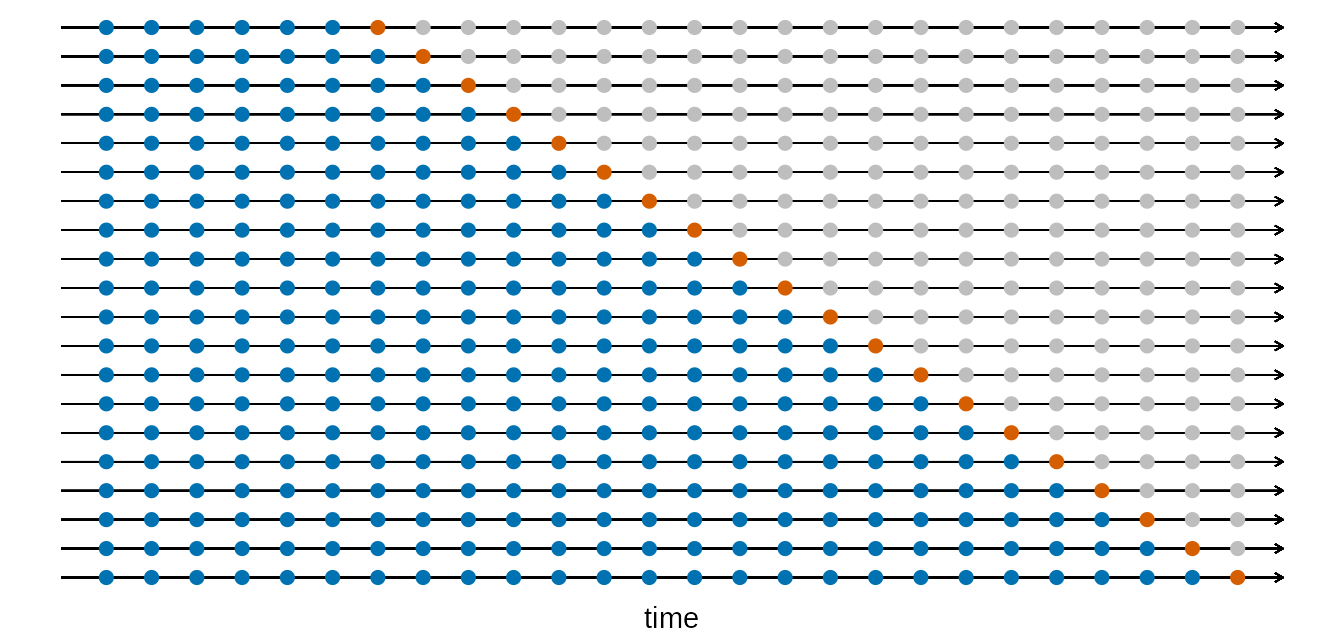
\includegraphics[width=\textwidth]{images/crossvalidationtimeseries.png}
    \caption{Cross validation for one step ahead timeseries data \cite{hyndman2018forecasting}}
    \label{fig:crossvalidationtimeseries}
\end{figure}
We then average all the observed losses in order to get an estimate for $Err$.
Notice, in the literature this procedure is sometimes also referred to evaluation on a rolling forecasting origin. This comes from the fact that at each iteration we push forward the origin of our forecast.
The same concept applies for multi step ahead forecasting, see Figure \ref{fig:crossvalidationtimeseries2}.
In predicting $\hat{y}_{N+m}$ we use as inputs $y_1, y_2, \dots, \hat{y}_{N},\hat{y}_{N+1},\dots, \hat{y}_{N+m-1}$, where $\hat{y}_{N},\hat{y}_{N+1},\dots, \hat{y}_{N+m-1}$ are one step ahead forecasts.
\begin{figure}
    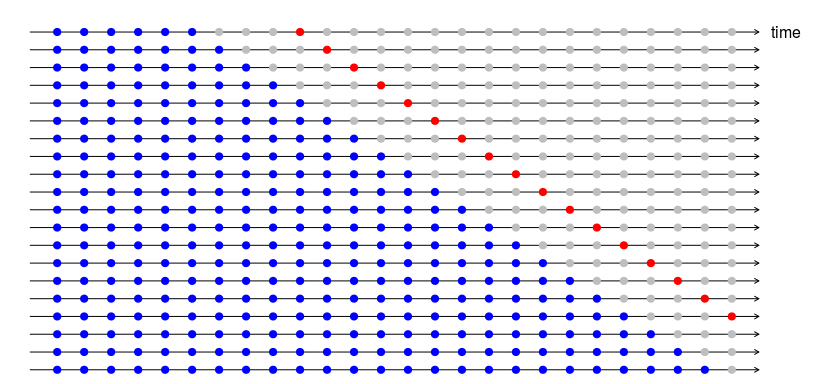
\includegraphics[width=\textwidth]{images/crossvalidationtimeseries2.png}
    \caption{Cross validation for m step ahead timeseries data \cite{hyndman2018forecasting}}
    \label{fig:crossvalidationtimeseries2}
\end{figure}

\section{Kernel methods best practices}
Following, are reported a couple of considerations important to keep in mind when working with kernel methods.

\subsection{Data normalization}\label{appendix:normalization}
With data normalization we transform the range of the feautures to a standard scale.
Such preprocessing step is essential when employing distance based algorithms like SVM or K-nearest neighbors. The rationale behind it is that by normalizing data we give an uniform weight to each feature in the learning process; in this way we do not favour larger scale features.
Examples of the most popular features scaling are:
\begin{itemize}
    \item Standard scaler= it computes the standard score $z$ of a sample $x$
    \\
    $z=\frac{x-\mu}{\sigma}$.
    \item MinMax scaler= it maps every data sample to the range $[0,1]$.
    \\
    $\frac{x-\min(X)}{\max(X)-\min(X)}$
    \item Robust scaler= it scales features using statistics that are robust to outliers.
    Essentially, it subtracts the median and then scales the data according to the interquantile range.
\end{itemize}
Many other data scaling algorithms exists, we refer the reader to a thorough comparison \citeW{scikitscalers}.
\\
We conclude this subsection with a custom example that motivates the need of feature scaling \citeW{scikitscale_example}. The idea is to compare the results of modelling the data with K-nearest neighbors on the unscaled data against the scaled data. The considered data is the wine recognition dataset \href{https://archive.ics.uci.edu/dataset/109/wine}{https://archive.ics.uci.edu/da-taset/109/wine}. The goal for this dataset is recognising from whose cultivator the wine comes based on two features with a completely different scale. The first feature has values in the [0,1000] range while the second feature has values contained in [1,10].
The unscaled and scaled version are compared in Figure \ref{fig:feature_scaler_example}.
\begin{figure}[!h]
    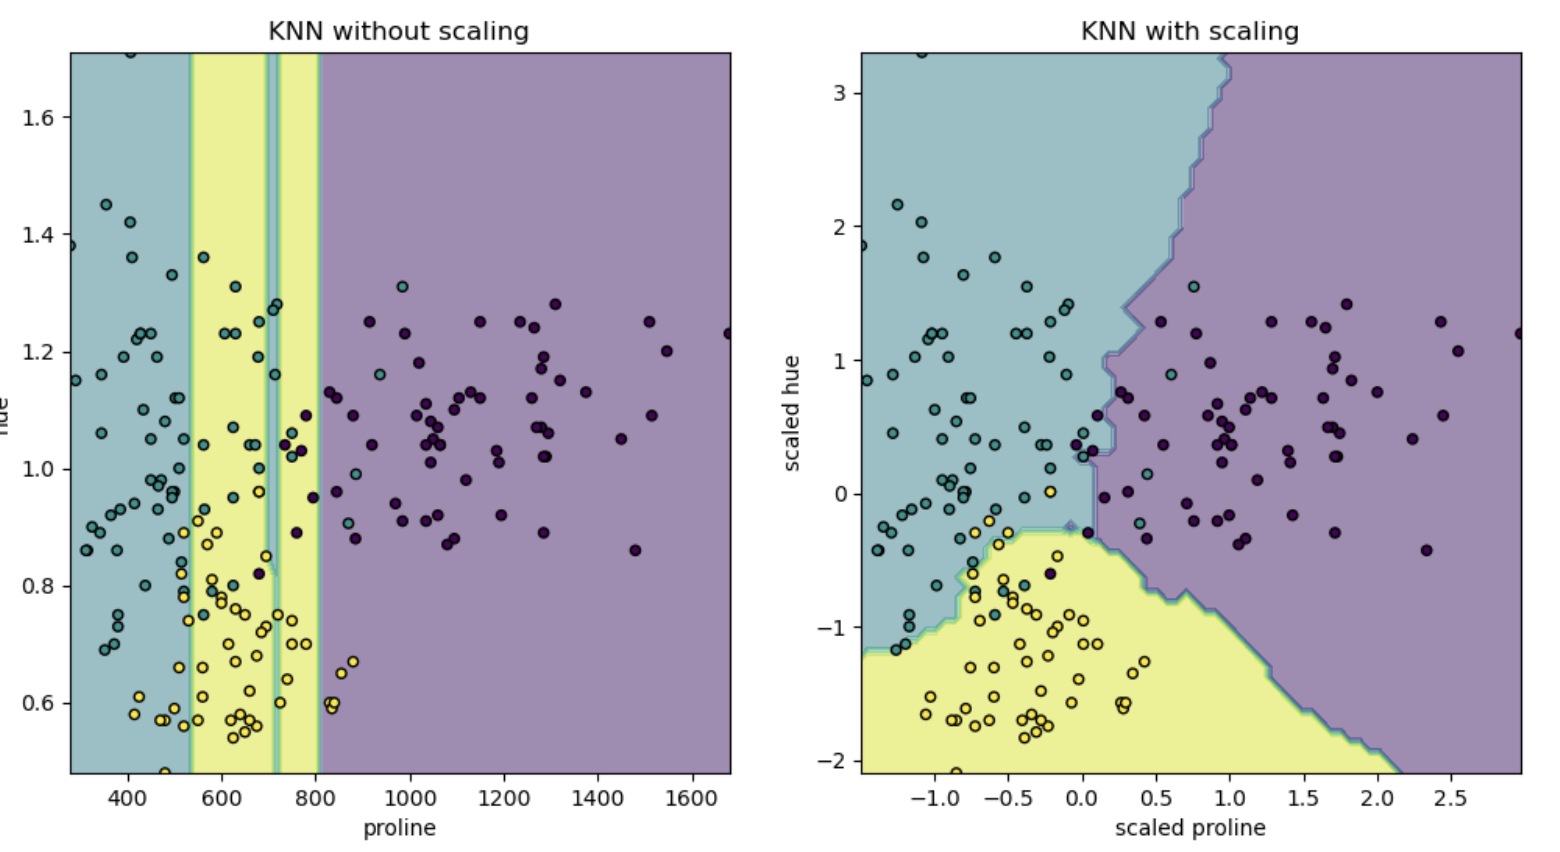
\includegraphics[width=\textwidth]{images/feature_scaler_example.png}
    \caption{Importance of feature scaling}
    \label{fig:feature_scaler_example}
\end{figure}
What we can conclude from the image is that, the model trained on scaled data is much better than the other.
On the left, we can see that distances between categories are impacted solely by the larger scale feature. Conversely, on the right, we have that the two features contribute equally in determining the neighbors.

\subsection{Data compression}
When the number of points $n$ is large, kernel methods suffer from high computational costs. 
Using kernel methods, we have that the storage cost is of the order $O(n^2)$ while the computational cost for finding the solution is of the order $O(n^3)$.
A significant speed up can be obtained thanks to low rank approximation.


\subsubsection{Nystrom decomposition}
The Nyström approximation involves storing a submatrix of the whole kernel matrix. Thus, storage and computational costs are reduced to $O(nm)$ and $O(nm^2)$ respectively.
Nyström works by selecting $m<n$ points, called representative points; it approximates $K$ as
\begin{equation}
    \tilde {K}=K_{n,m} K_{m,m}^{-1}K_{n,m}^\intercal
\end{equation}


\subsubsection{Pivoted Cholesky decomposition}
Pivoted Cholesky approximates the Cholesky decomposition of a matrix. Since kernel matrices are positive definite, they can be decomposed in terms of the Cholesky decomposition. Hence, we have that pivoted Cholesky can be used to approximate the full kernel matrix.


\newpage
\section{Source code}\label{src_code}
The whole code for the project is hosted on
\url{https://github.com/luca-pernigo/ThesisKernelMethods}\label{github_repo}.
\\
\begin{itemize}
    \item query/: folder containing Scopus data and scripts to generate bibliometric survey plots in Section \ref{literature_review}.
    \item thesis/: folder containing tex files for thesis.
    \item beamer/: folder containing tex files for pptx thesis defence.
    \item experiments: folder containing train, test script for each of the experiments carried out in the thesis alongside with the binary files of the pickled models.
    \item experiments/src/kernel\_quantile\_regression/kqr.py: file implementing our custom kernel quantile regression.
    \item experiments/Data: cleaned data used in our experimental studies.
    \item experiment/plots/: folder storing plots resulting from experiments.
    \item experiment/eda/: scripts for exploratory data analysis.
    \item experiments/point/: scripts for experiments point framework.
    \item experiments/train\_test/: scripts for training, testing and generating tables for experiments probabilistic framework.
    \item experiments/utils/: utility functions used in extracting, transforming and cleaning raw data.
    \item extradata/: folder containing data for experiments in section \ref{appendix:quantile_regressor_extensive_comparison}.
    \item requirements.txt: pip freeze of python packages used.
\end{itemize}
